\subsection{Крайно произведение}
\label{subsect:domains:product}
\index{област на Скот!крайно произведение}
\marginpar{\cite[стр. 125]{winskel}}

Да разгледаме тройките $\A_i = (A_i, \sqsubseteq_i, \bot_i)$, където $i = 1,\dots,n$. Дефинираме тройката 
$\prod^n_{i=1}\A_i = (A, \sqsubseteq, \bot)$ като:
\begin{itemize}
\item
  $A \df A_1\times\dots\times A_n$, декартовото произведение на множествата $A_1,\dots,A_n$;
\item 
  $\pair{a_1,\dots,a_n} \sqsubseteq \pair{b_1,\dots,b_n} \dfff a_1 \sqsubseteq_1 b_1\ \&\ \dots\ \&\ a_n \sqsubseteq_n b_n$,
  която ще наричаме {\em поточкова наредба};
\item
  $\bot \df \pair{\bot_1,\dots,\bot_n}$.
\end{itemize}

\begin{framed}
  \begin{proposition}
    \label{pr:cartesian}
    Ако $\A_1,\dots,\A_n$ са области на Скот, то $\prod^n_{i=1}\A_i$ е област на Скот.
  \end{proposition}  
\end{framed}
\begin{hint}
  Лесно се съобразява, че $\sqsubseteq$ е частична наредба и че $\bot$ е най-малкият елемент.
  Да разгледаме една верига $\chain{\ov{a}}{i}$ в $\prod^n_{i=1}\A_i$,
  където $\bar{a}_i = \pair{a^i_1,\dots,a^i_n}$.
  Да положим \[\bar{a} \df \pair{\bigsqcup_i a^i_1,\bigsqcup_i a^i_2,\ldots,\bigsqcup_i a^i_n,}.\]
  Ще докажем, че $\bar{a}$ е точната горна граница на верига $\chain{\ov{a}}{i}$, т.е.
  \[\bigsqcup_i\bar{a}_i = \pair{\bigsqcup_i a^i_1,\bigsqcup_i a^i_2,\ldots,\bigsqcup_i a^i_n,}.\]
  Това ще направим на две стъпки.
  \begin{itemize}
  \item 
    Първо ще докажем, че $\bar{a}$ е горна граница на $\chain{\bar{a}}{i}$.
    За всеки индекс $j$, имаме, че $\bar{a}_j = (a^j_1,\dots,a^j_n)$.
    Да разгледаме $1 \leq k \leq n$.
    Ясно е, че $a^j_k \sqsubseteq_k \bigsqcup_i a^i_k$.
    Оттук веднага следва, че
    \[\bar{a}_j = \pair{a^j_1,\dots,a^j_n} \sqsubseteq \pair{\bigsqcup_i a^i_1,\dots,\bigsqcup_i a^i_n} = \bar{a}.\]
  \item
    Нека $\bar{b} = \pair{b_1,\dots,b_n}$ е произволна горна граница на $\chain{\bar{a}}{i}$.
    Ще докажем, че $\bar{a} \sqsubseteq \bar{b}$.
    Знаем, че за всеки индекс $j$, $\bar{a}_j \sqsubseteq \bar{b}$.
    Да разгледаме произволен индекс $k$, за който $1 \leq k \leq n$.
    Знаем, че в областта на Скот $\A_k$ е изпълнено, че $a^j_k \sqsubseteq_k b_k$, за всеки индекс $j$.
    Оттук следва, че $b_k$ е горна граница за веригата $(a^j_k)^\infty_{j=0}$ в $\A_k$.
    Следователно
    \[\bigsqcup_j a^k_j \sqsubseteq_k b_k.\]
    Заключаваме, че
    \[\bar{a} = \pair{\bigsqcup_i a^i_1,\dots,\bigsqcup_i a^i_n} \sqsubseteq \pair{b_1,\dots,b_n} = \bar{b}.\]
  \end{itemize}
\end{hint}

\begin{framed}
  \begin{figure}[H]
    \centering
    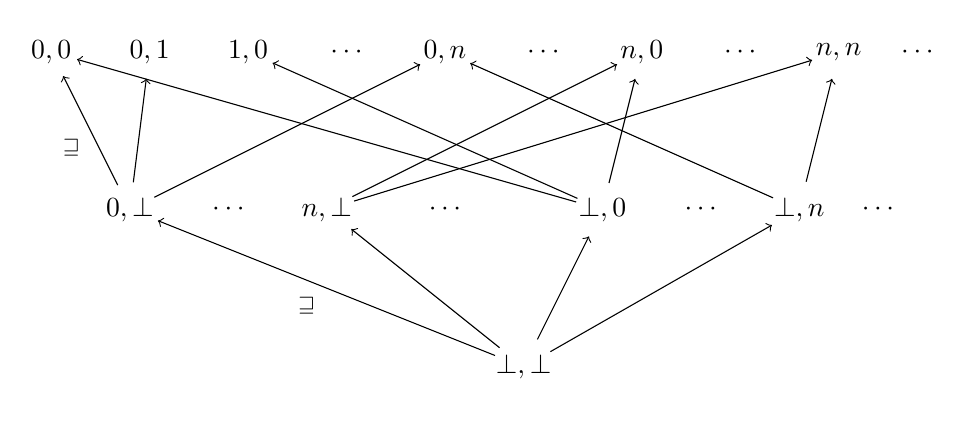
\begin{tikzpicture}[shorten >=1pt,->]
      \tikzstyle{vertex}=[circle,minimum size=17pt,inner sep=0pt]
      
      \node[vertex] (bot) at (5,-1) {$\pair{\bot,\bot}$};
      
      \node[vertex] (0b) at (0,1) {$\pair{0,\bot}$};
      \node[vertex] (db) at (1.25,1) {$\cdots$};
      \node[vertex] (nb) at (2.5,1) {$\pair{n,\bot}$};
      \node[vertex] (ddb) at (4,1) {$\cdots$};
      
      \node[vertex] (b0) at (6,1) {$\pair{\bot,0}$};
      \node[vertex] (bd) at (7.25,1) {$\cdots$};
      \node[vertex] (bn) at (8.5,1) {$\pair{\bot,n}$};
      \node[vertex] (bdd) at (9.5,1) {$\cdots$};
      
      \node[vertex] (00) at (-1,3) {$\pair{0,0}$};
      \node[vertex] (01) at (0.25,3) {$\pair{0,1}$};
      \node[vertex] (10) at (1.5,3) {$\pair{1,0}$};
      \node[vertex] (ddd) at (2.75,3) {$\cdots$};
      \node[vertex] (0n) at (4,3) {$\pair{0,n}$};
      \node[vertex] (dddd) at (5.25,3) {$\cdots$};
      \node[vertex] (n0) at (6.5,3) {$\pair{n,0}$};
      \node[vertex] (ddddd) at (7.75,3) {$\cdots$};
      \node[vertex] (nn) at (9,3) {$\pair{n,n}$};
      \node[vertex] (dddddd) at (10,3) {$\cdots$};

      \draw (bot) -- node[below left]{$\scriptstyle{\sqsupseteq}$} (0b);
      \draw (bot) -- (nb);
      \draw (bot) -- (b0);
      \draw (bot) -- (bn);

      \draw (0b) -- node[below left]{$\scriptstyle{\sqsupseteq}$} (00);
      \draw (0b) -- (01);
      \draw (0b) -- (0n);

      \draw (b0) -- (00);
      \draw (b0) -- (10);
      \draw (b0) -- (n0);
      \draw (nb) -- (n0);
      
      \draw (nb) -- (nn);
      \draw (bn) -- (0n);
      \draw (bn) -- (nn);

    \end{tikzpicture}    
    \caption{Графично представяне на част от $\sqsubseteq$ върху $\Nat^2_\bot$}
    \label{fig:flat-nat-2}
  \end{figure}
\end{framed}

Вижда се от \Fig{flat-nat-2}, че всяка верига в $\Nat^2_\bot$ има дължина най-много $3$.
Лесно се съобразява, че всяка верига в $\Nat^k_\bot$ има дължина най-много $k+1$.
Свойството, че всяка верига в $\Nat^k_\bot$ има само краен брой различни члена
ще се окаже важно по-нататък. Сега ще въведем понятие, което описва това свойство в произволна област на Скот.
\marginpar{ $\Nat^k_\bot = \underbrace{\Nat_\bot \times \cdots \times\Nat_\bot}_{k}$}

Нека $\A$ е област на Скот и да разгледаме една верига $\chain{a}{n}$ в $\A$.
Ще казваме, че $\chain{a}{n}$ се {\bf стабилизира}, ако съществува индекс $n_0$, за който
\[(\forall n \geq n_0)[a_{n_0} = a_{n}],\]
т.е.
\[a_0 \sqsubseteq a_1 \sqsubseteq a_2 \sqsubseteq \cdots \sqsubseteq a_{n_0} = a_{n_0+1} = a_{n_0+2} = \cdots\]
От казаното по-горе следва, че всяка растяща верига в $\Nat^k_\bot$ се стабилизира.

\begin{remark}
  Едни от основните области на Скот, които ще разглеждаме при дефинирането на денотационната семантика
  ще бъдат $\Nat_\bot$ и $\Nat^k_\bot$.
\end{remark}


%%% Local Variables:
%%% mode: latex
%%% TeX-master: "../sep"
%%% End:
